\section{Generalità sui bacini e sull'evento pluviometrico di studio}
I bacini montani, interessati dallo studio di questa relazione, sono due classici esempi di unità geomorfologiche montane.\\
Infatti, riguardano rispettivamente i bacini idrogeologici dei fiumi Boite \cite{fiume_boite} e Piave \cite{fiume_piave}, posti nel territorio bellunese.
\begin{figure}[H]
    \begin{minipage}[]{7cm}
        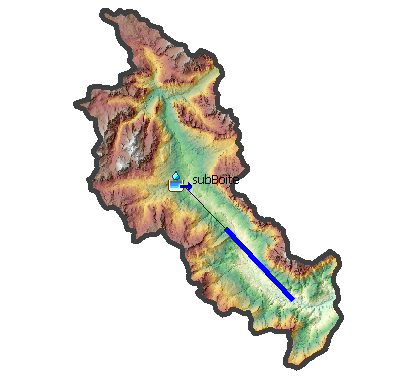
\includegraphics[scale=0.73]{immagini/bac_boite.PNG}
        \caption{Bacino idrografico del Boite.}
    \label{bacino_boite}    
    \end{minipage}
        \hspace{2cm}
    \begin{minipage}[]{7cm}
        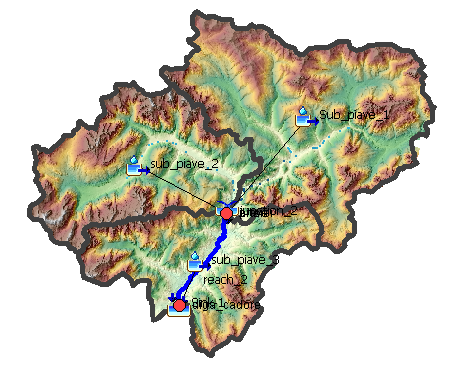
\includegraphics[scale=0.75]{immagini/bac_piave.PNG}
        \caption{Bacino idrografico del Piave.}
    \label{bacino_piave}
    \end{minipage} 
        \end{figure}

Al fine di svolgere in modo più corretto la procedura di analisi spaziale (come verrà descritta successivamente), si è scelto di suddividere il territorio del bacino del Piave in ulteriori tre sottobacini.\\
Il bacino del fiume Boite ha un'estensione di 383 $km^2$, mentre il bacino del Piave ha un'estensione totale di 813 $km^2$.\\
